\artigofalse
\chapter{R-package spsann: Optimization of Sample Configurations using Spatial 
Simulated Annealing}
\label{apen:spsann}

% 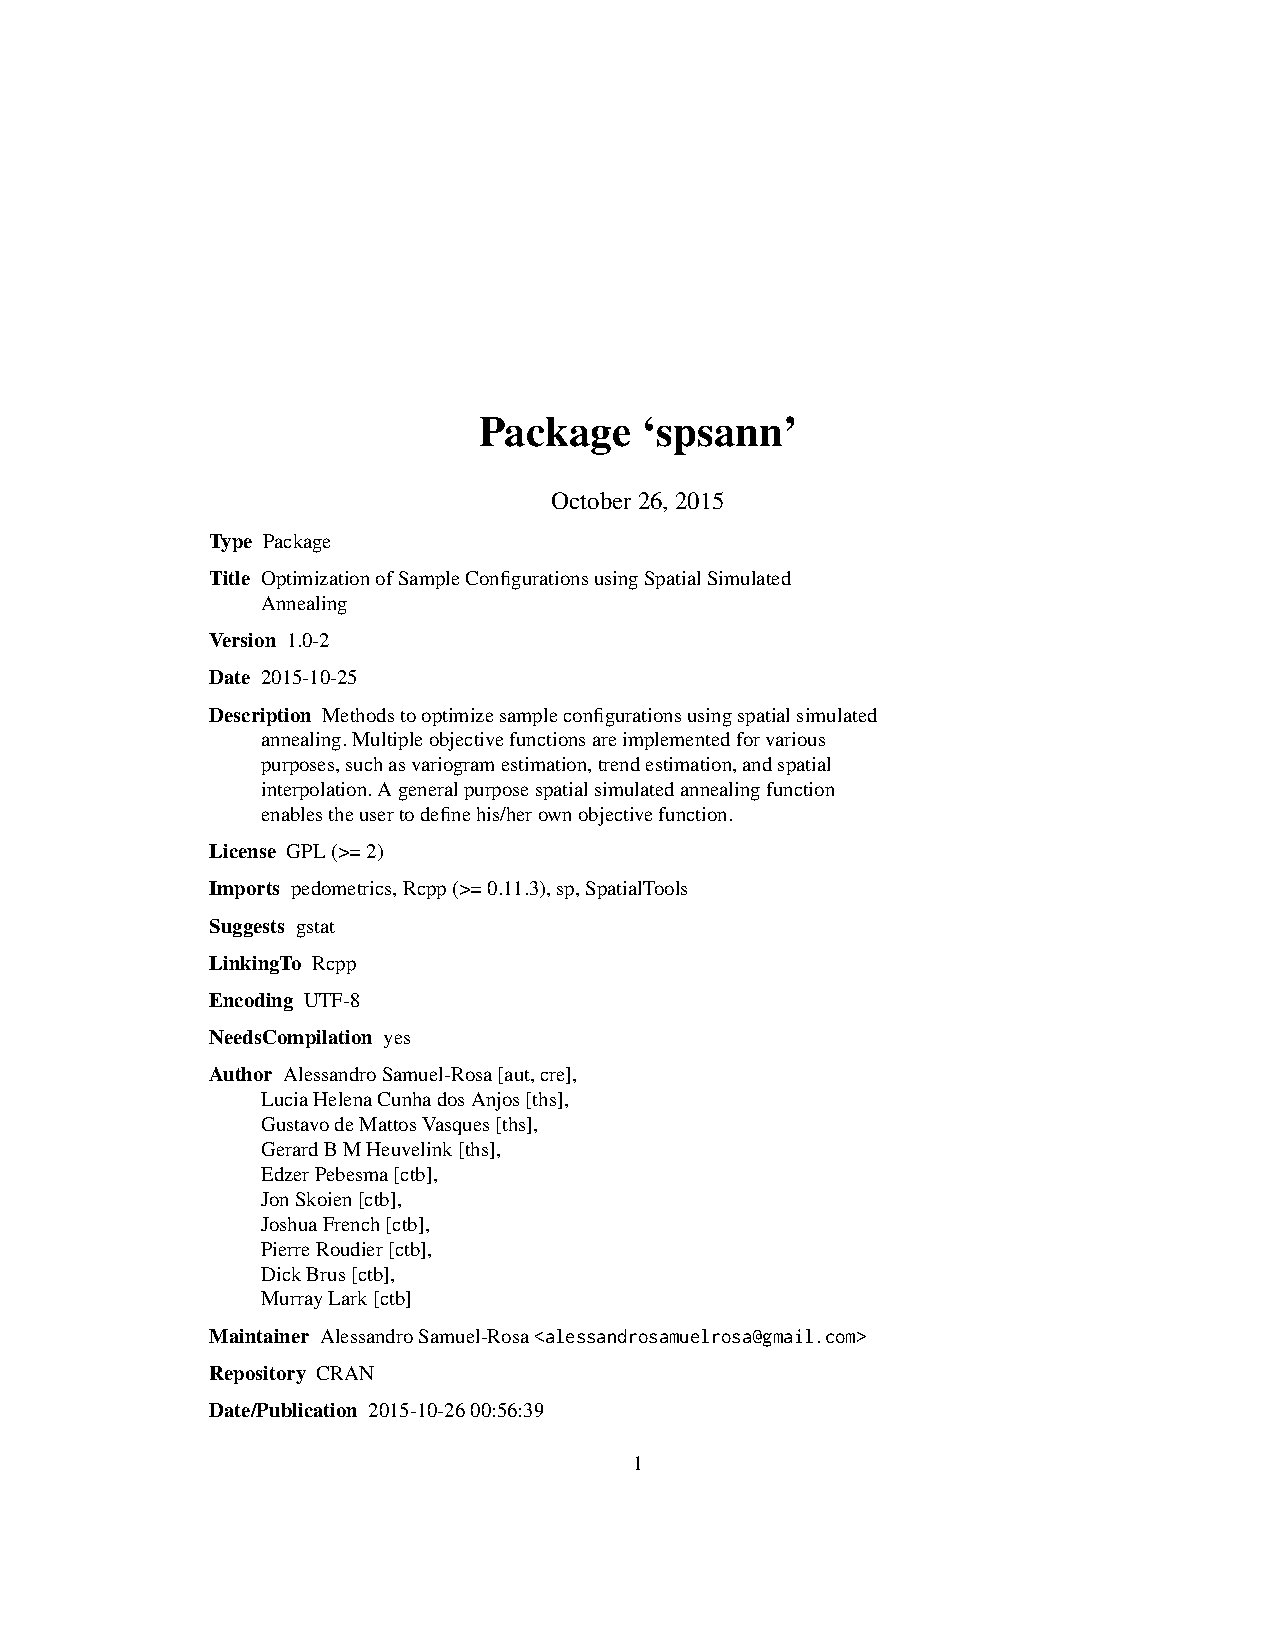
\includepdf[pages=-,pagecommand={}]{chap/spsann.pdf}

\section{Objective functions}



\section{Spatial Simulated Annealing}

\subsection{Generation Mechanism}

The \textit{generation mechanism} corresponds to the set of formal rules used 
to randomly perturb the sample configuration to create a new solution out of the
current one. This is done by adding random noise to the coordinates of one of 
the sample points, a process known as \textit{jittering}.

Before we jitter a given sample point, we have to define the maximum quantity 
of random noise that can be added to its coordinates, i.e. the area within 
which it can be moved around. In principle, this area corresponds to a rectangle
centred at the sample point that ignores the presence of non-sampling areas 
(e.g. buildings and water bodies) and the finiteness of the sampling region. We 
call this the \textit{search graph}.

Once we know the size of the search graph, we have to decide upon how much 
noise will be added to the coordinates of our sampling point, i.e. to choose a
candidate location. This can be done in two different ways. We can use an 
\textit{infinite} set of candidate locations, that is, any location within the 
search graph can be selected as the candidate location for our sample point. 
After a candidate location is selected, we check if it falls within the sampling
region but does not fall within a non-sampling area. These checks usually are 
computationally demanding, the reason why this method is not implemented in 
the \textbf{spsann}-package.

A more efficient way of selecting a candidate location is to first identify the
set of \textit{effective} candidate locations for our sample point. This can be
done using a \textit{finite} set of candidate locations. A finite set of 
candidate locations is created by discretizing the sampling region beforehand, 
that is, creating a fine grid of points that serve as candidate locations during
the entire search for the optimum sample configuration. This is the least 
computationally demanding jittering method because, by definition, the candidate
location will always fall within the sampling region and out of non-sampling 
areas.

Using a finite set of candidate locations has two main disadvantages. First, not
all locations in the sampling region can enter the sample. The sample points are
limited to a finite set of regularly spaced candidate locations which is not 
guaranteed to include the \textit{true} global optimum configuration. Second, 
when a sample point is jittered, it may be that the selected candidate location
is occupied by a sample point. When this happens, another candidate location 
has to be sought because we cannot have more than one point at the same 
location. In the worst case, most (or all) candidate locations are occupied by 
a sample point, demanding an iterative search for, say, as long as there are 
points in the sample. In general, the more points there are in the sample (or 
the smaller the size of the search graph -- see bellow), the more likely it is 
that the selected candidate location already is occupied by a sample point. If 
a solution is not found in a reasonable amount of time, our sample point is 
kept in its original location.

The \textbf{spsann}-package uses a more elegant method based on using a finite
set of candidate locations coupled with a form of \textit{two-stage random 
sampling} as implemented in the \texttt{spsample}-function of the 
\textbf{spcosa}-package.

 Because 
the candidate locations are placed on a finite regular grid, they can be 
seen as being the centre nodes of a finite set of grid cells (or pixels of 
a raster image). In the first stage, one of the 'grid cells' is selected 
with replacement, i.e. independently of already being occupied by 
another sample point. The new location for the point chosen to be jittered 
is selected within that 'grid cell' by simple random sampling. This 
method guarantees that \textit{almost} any location in the sampling region can 
be a candidate location. It also discards the need to check if the new 
location already is occupied by another point, simplifying the code and 
(possibly) speeding up the computations.
 
The size of the search graph
is reduced linearly at the end of each Markov chain. The size of the search 
graph is correlated with the concept of \textit{temperature}: a larger search 
graph is equivalent to higher temperatures, which potentially result in more 
movement or 'agitation' of the set of points.

\begin{equation}
  x_max = x_max0 - (chains_i / chains) * (x_max0 - x_min) + x_cellsize
  
  y_max = y_max0 - (chains_i / chains) * (y_max0 - y_min) + y_cellsize
\end{equation}

where $x_max0$ and $y_max0$ are the maximum allowed shifts in the x- and 
y-coordinates in the first chain, $x_min$ and $y_min$ are the minimum 
required shifts in the x- and y-coordinates, $x_max$ and $y_max$ are the
maximum allowed shifts in the x- and y-coordinates during the next chain, 
$chains$ and $chain_i$ are the total and current chains, and $x_cellsize$ and
$y_cellsize$ are the grid spacing in the x- and y-coordinates.

\subsection{Annealing Schedule}

The \textit{annealing schedule} corresponds to a set of formal rules that 
determine how the probability of accepting inferior system configurations is 
decreased as the search for the globally optimum system configuration evolves.
